% Copyright (c) 2014,2016 Casper Ti. Vector
% Public domain.

\chapter{HybriG的系统架构概述}
为了更好地应对含有大量重边的属性图应用场景,规避传统图数据库的局限性,本文提出了一种复合存储架构HybriG。HybriG架构应用在明略数据的关联数据分析平台SCOPA中,提供属性图数据的查询与存储。
HybriG将图的连接信息和点集的属性数据存储在Titan中,边集的所有属性数据则直接存储在HBase中。由于HybriG架构基于Titan和HBase实现存储,而Titan的数据本身也存储在HBase中,为了方便表述以及避免混淆,下文中的HBase指的都是不包含Titan数据表的部分。Titan在HBase中的数据表直接用Titan代称。

\begin{figure}[htbp]
\centering
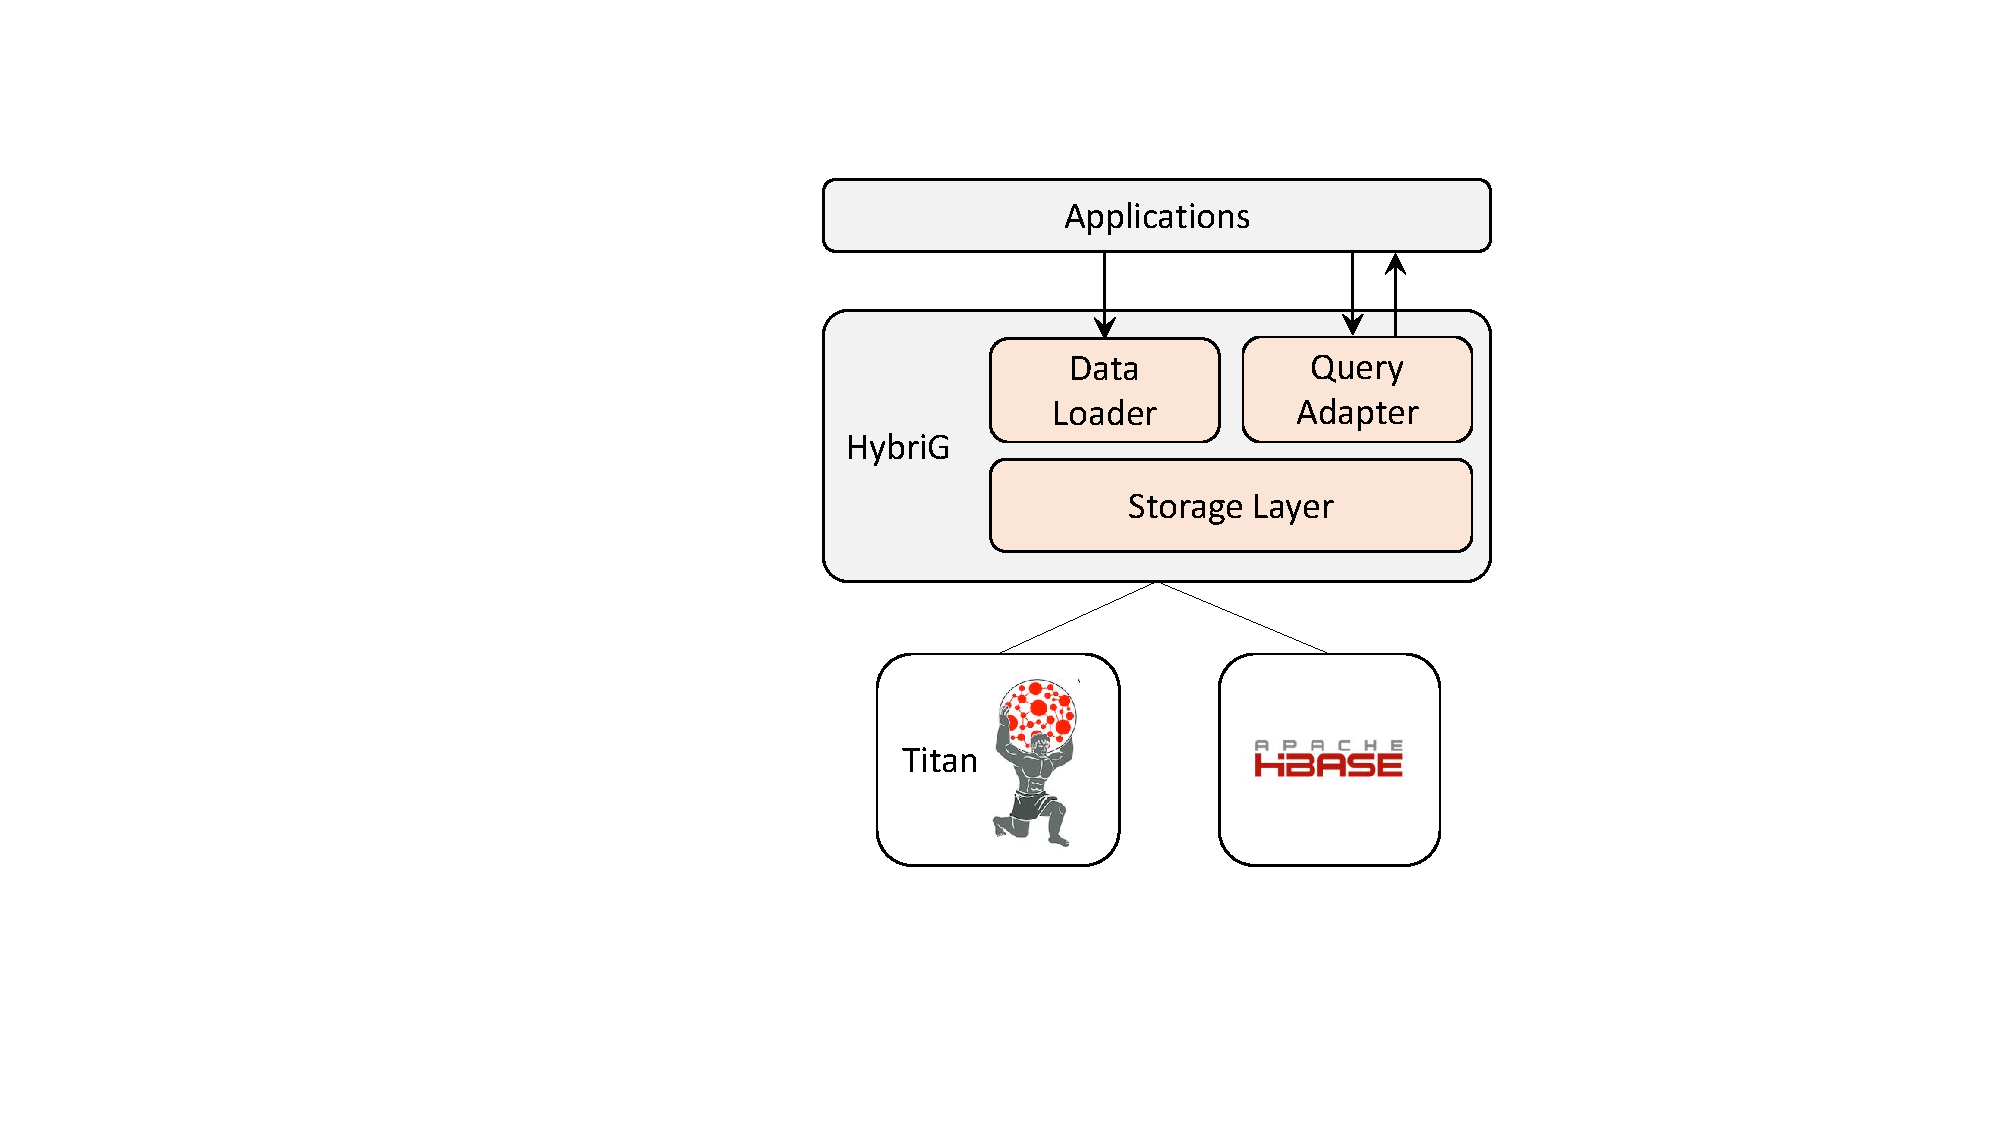
\includegraphics[height=80mm]{fig/arch.pdf}
\caption{HybriG系统架构}
\label{fig:arch}
\end{figure}

图 \ref{fig:arch}展示了HybriG的系统架构。Storage Layer是HybriG的存储层,Query Adapter和Data Loader分别为用户程序提供图查询和数据插入接口。其中,Query Adapter将图查询转换为对Titan和HBase数据的高效查询,再将结果汇总返回给用户程序。Data Loader实现了数据的高效导入,在面对大批量的数据导入时,实现了错误恢复、断点恢复机制,同时保证了Titan和HBase的数据一致性。下面将分别介绍HybriG各模块的实现。


% vim:ts=4:sw=4
